% Created 2026-04-15 Wed 12:19
% Intended LaTeX compiler: pdflatex
\documentclass[11pt]{article}
\usepackage[utf8x]{inputenc}
\usepackage[T1]{fontenc}
\usepackage{graphicx}
\usepackage{longtable}
\usepackage{wrapfig}
\usepackage{rotating}
\usepackage[normalem]{ulem}
\usepackage{amsmath}
\usepackage{amssymb}
\usepackage{capt-of}
\usepackage{hyperref}
\usepackage{minted}
\usepackage{parskip}
\graphicspath{{./images/}{./assets/}}
\usepackage[labelformat=simple]{subcaption}
\renewcommand\thesubfigure{(\alph{subfigure})}
\usepackage[date=year,%
backend=biber,%
style=alphabetic,%
maxnames=5,%
minnames=3,%
maxalphanames=4,%
minalphanames=3,%
backref=true,%
doi=false,%
isbn=false,%
url=false,%
eprint=false]{biblatex}
\DefineBibliographyStrings{english}{%
backrefpage  = {\lowercase{s}ee p.}, % for single page number
backrefpages = {\lowercase{s}ee pp.} % for multiple page numbers
}
\addbibresource{/home/bvraghav/bibliography.bib}
\hypersetup{
colorlinks,
allcolors=.,
urlcolor=blue,
citecolor=gray,
linkcolor=red,
}
\usepackage{ragged2e}
\usepackage{tabularx}
\usepackage{enumitem}
\setlist{noitemsep}
\usepackage{parskip}
\usepackage[a4paper,margin=1.5in]{geometry}
\usepackage{xfrac}
\setcounter{secnumdepth}{3}
\author{Raghav B. Venkataramaiyer}
\date{Apr '26}
\title{Introduction to AR}
\hypersetup{
 pdfauthor={Raghav B. Venkataramaiyer},
 pdftitle={Introduction to AR},
 pdfkeywords={},
 pdfsubject={},
 pdfcreator={Emacs 30.2 (Org mode 9.7.11)}, 
 pdflang={English}}
\begin{document}

\maketitle
\setcounter{tocdepth}{2}
\tableofcontents

Welcome to the frontier of Augmented Reality (AR).

Unlike Virtual Reality (VR), which creates a completely
synthetic environment, AR ``augments'' the physical world
by overlaying digital data onto it.

To understand AR at a professional level, you have to
look past the filters and games; it is essentially a
high-speed optimization problem involving geometry,
optics, and data processing.
\section{System Structure of Augmented Reality}
\label{sec:org36551f4}
The structure of an AR system is defined by a
continuous feedback loop between the physical
environment and the digital processor.
\subsection{The Core Components}
\label{sec:org63a975a}

\begin{description}
\item[{Sensing and Tracking}] The system must ``see'' the
world. This involves hardware (cameras, LIDAR, IMUs)
capturing the 3D structure and the user's pose
(position and orientation).
\item[{Processing Unit}] The ``brain'' (CPU/GPU/NPU) that
calculates the spatial relationship between the user
and the environment.
\item[{Digital Content Generator}] The engine (like Unity
or Unreal) that renders the 3D models or data.
\item[{Display/Output}] The medium where the real and
virtual worlds merge. This can be \emph{Optical
See-Through} (like HoloLens), \emph{Video See-Through}
(like a smartphone screen), or \emph{Spatial AR}
(projectors).
\end{description}
\section{Key Technologies in AR}
\label{sec:orgcbbf493}

\subsection{SLAM (Simultaneous Localization and Mapping)}
\label{sec:orge91ff18}
This is the ``holy grail'' of AR. It allows a device to
build a map of an unknown environment while
simultaneously keeping track of its own location within
that map.
\subsection{Computer Vision (CV)}
\label{sec:org4dadbb7}
CV algorithms are used for object recognition, plane
detection (finding a floor or table), and
``occlusion''---the ability for a digital object to be
hidden behind a physical one.
\section{The Academic Grounding}
\label{sec:orgcdd5b0b}

\subsection{Mathematics : The Language of Space}
\label{sec:orge10ded4}
AR is built on \emph{Linear Algebra} and \emph{Projective
Geometry}. To place a digital teapot on your real desk,
the system performs coordinate transformations.
\subsubsection{Matrix Transformations}
\label{sec:orgacc8812}
We use \(4 \times 4\) matrices to represent rotation,
translation, and scaling in 3D space
\subsubsection{Pinhole Camera Model}
\label{sec:pin-hole-camera-model}
This relates a 3D world point \(\mathbf{m};
\mathbf{m}^{\top} \equiv \begin{bmatrix} x & y & z
\end{bmatrix}\) to a 2D image point
\(\overline{\mathbf{z}};
\overline{\mathbf{z}}^{\top}\equiv \begin{bmatrix} u &
v \end{bmatrix}\) using a projection function \(h\):

\begin{align*}
  \overline{\mathbf{z}}
  &= h(\mathbf{m}; \boldsymbol{\mu}) \\
  \exists s \text{ scalar, so that, }\quad
  s \overline{\mathbf{z}}
  &= K [R | \mathbf{t}] \begin{bmatrix}
    \mathbf{m} \\ 1
  \end{bmatrix}
\end{align*}

where,
\begin{itemize}
\item \(K\) represents intrinsic parameters (focal length,
etc.)
\item \([R | \mathbf{t}]\) represents extrinsic parameters
(rotation and translation) that are computed using
the camera pose in parameterised state vector
\(\boldsymbol{\mu}\).  See also:
\S~\ref{sec:state-vector}.
\end{itemize}
\subsubsection{Quaternions}
\label{sec:orgc29380d}
Used instead of Euler angles to handle 3D rotations
without ``gimbal lock'' and with higher computational
efficiency.
\paragraph*{Cheatsheet}
\label{sec:org62909e1}
Quaternions are 4D Complex Numbers.

\begin{align*}
  \mathbf{q}
  &= w + x\imath + y\jmath + zk
  &&\equiv \begin{bmatrix}
      w & x & y & z
  \end{bmatrix}^{\top} \equiv \begin{bmatrix}
      w \\ \mathbf{v}
  \end{bmatrix}
  \\
  \|\mathbf{q}\|_F^2
  &= w^2 + x^2 + y^2 + z^2 = 1
  && \text{Unit Quaternion for rotation.}
  \\
  w
  &= \cos\frac{\theta}{2} \quad
    \mathbf{v} = \sin\frac\theta2 \mathbf{u}
  && \text{Rotation by } \theta \text{ around unit
     vector } \mathbf{u}.
  \\
  \imath\jmath k
  &= \imath^2 = \jmath^2 = k^2 = -1
  && \text{Quaternion multiplication rules.}
  \\
  \mathbf{q}_{\text{new}}
  &= \mathbf{q}_1 \otimes \mathbf{q}_2
  && \text{Rotation } \mathbf{q}_1 \text{ followed by }
     \mathbf{q}_2
\end{align*}

Quaternion to Rotation Matrix:
\begin{align*}
  R
  &= \begin{bmatrix}
    1 - 2(y^2 + z^2) & 2(xy - wz) & 2(xz + wy) \\
    2(xy + wz) & 1 - 2(x^2 + z^2) & 2(yz - wx) \\
    2(xz - wy) & 2(yz + wx) & 1 - 2(x^2 + y^2)
  \end{bmatrix}
\end{align*}
\paragraph*{Advantages}
\label{sec:org91baea6}
One might wonder why we don't just optimize the 9
numbers in the \(3 \times 3\) matrix directly in our
Quadratic Program.

\begin{enumerate}
\item \emph{Constraint Satisfaction}: A rotation matrix has 9
numbers but only 3 ``degrees of freedom.''  Keeping a
matrix orthogonal during optimization is hard.
Keeping a quaternion at unit length is easy (just
divide by the norm).
\item \emph{Smoothness}: If we need to estimate the camera
position between two frames (interpolation),
quaternions allow for SLERP (Spherical Linear
Interpolation), which creates smooth, realistic
motion blur and tracking.
\item \emph{Efficiency}: Multiplying two quaternions (combining
two rotations) takes only 16 multiplications, while
multiplying two \(3 \times 3\) matrices takes 27.
\end{enumerate}
\subsection{CS : The Engine of Interaction}
\label{sec:org02c3eea}
From a CS perspective, AR is a challenge of latency and
real-time rendering.
\subsubsection{Graphics Pipeline}
\label{sec:orgdeb6d56}
Understanding how vertices are processed into
pixels. To maintain immersion, the ``motion-to-photon''
latency must be under 20ms; otherwise, the user
experiences motion sickness.
\subsubsection{Algorithms}
\label{sec:org843b240}

Spatial indexing (like Octrees or KD-trees) is used to
quickly calculate collisions between digital objects
and the physical world map.
\subsubsection{Optimization}
\label{sec:org9e52716}

Since many AR devices are mobile, code must be highly
optimized for thermal and battery constraints, often
moving heavy CV tasks to specialized DSPs (Digital
Signal Processors).
\subsection{IT : The Infrastructure}
\label{sec:org00ee334}
AR doesn't exist in a vacuum; it requires a robust IT
backbone to function at scale.
\subsubsection{Edge Computing \& 5G}
\label{sec:orgb91c32a}
Rendering complex 3D models can be too taxing for a
headset.  IT infrastructure uses ``Edge'' servers to do
the heavy lifting and beam the frames back via
low-latency 5G.
\subsubsection{Cloud Anchors}
\label{sec:orge2e400e}
This allows ``persistent AR.''  If I leave a digital note
on a wall, IT protocols ensure that when you walk by an
hour later, your device retrieves that specific spatial
data from the cloud and renders the note in the exact
same spot.
\subsubsection{Data Security}
\label{sec:org9ed03a0}
AR devices are essentially ``roving surveillance'' tools,
capturing constant video and spatial maps. The IT
challenge is securing this ``Spatial Data'' to protect
user privacy.
\section{EKF SLAM}
\label{sec:org4b775b5}

Simultaneous Localisation and Mapping \\
with Extended Kalman Filter.

At its core, SLAM is a ``chicken-and-egg'' problem:
\begin{itemize}
\item to map the environment, we need to know the location;
\item to know the location, we need a map.
\end{itemize}

We resolve this using state estimation.  The system
maintains a \emph{Gaussian distribution} over the state.
That is to say that it isn't just a single point, but a
stochastic entity, with
\begin{itemize}
\item mean vector \(\boldsymbol{\mu}\) (where we think we
are), and
\item a covariance matrix \(\Sigma\) (how uncertain we are).
\end{itemize}

The \emph{Extended Kalman Filter} (EKF) was historically the
standard for SLAM.  It treats the problem as a series
of predictions and corrections.

\begin{description}
\item[{Prediction Step}] Uses a motion model to guess the
new state based on sensors like accelerometers.
\item[{Correction Step}] Uses a measurement model to
compare what the camera sees vs. what it expected to
see based on the map.
\end{description}

Because the real world is non-linear (rotations involve
sines and cosines), we use the Jacobian matrix \(H\) to
linearize these functions at the current estimate.  The
Jacobian represents the partial derivatives of the
frame with respect to the state:

\begin{align*}
  H &= \frac{\partial \mathbf{z}} {\partial
      \boldsymbol{\mu}}
\end{align*}
\subsection{The State Vector}
\label{sec:state-vector}
In SLAM, we define a state vector \(\boldsymbol{\mu}_t\)
that contains both the robot's pose, \emph{i.e.} position
\(\mathbf{p}; \mathbf{p}^{\top} \equiv \begin{bmatrix} x
& y & z \end{bmatrix}\)
 plus orientation quaternion
\(\mathbf{q}; \mathbf{q}^{\top} \equiv \begin{bmatrix}
q_w&q_x&q_y&q_z \end{bmatrix}\); and the coordinates of
all landmarks \(\{\mathbf{m}_1, \mathbf{m}_2, \dots, \mathbf{m}_n\}\) discovered so
far:

\begin{align*}
  \boldsymbol{\mu}_t
  &= \left[ \underbrace{x, y, z,
q_w, q_x, q_y, q_z}_{\text{Camera Pose}},
\underbrace{m_{1,x}, m_{1,y}, m_{1,z}, \dots,
m_{n,z}}_{\text{Map Landmarks}} \right]^{\top}
\end{align*}

A 3D AR camera gives us a 2D projection \(\mathbf{z};
\mathbf{z}^{\top} \equiv \begin{bmatrix} u & v
\end{bmatrix}\) of a 3D landmark \(\mathbf{m};
\mathbf{m}^{\top} \equiv \begin{bmatrix} m_x&m_y&m_z
\end{bmatrix}\).  Also, typically, the device has an
Inertial Measurement Unit (IMU).  We use the integrated
accelerations and angular velocities as the control
input \(\mathbf{u}\).

The goal is to find the posterior probability of the
state given all observations \(\mathbf{z}\) and control
inputs \(\mathbf{u}\):

\begin{align*}
  P \left(\boldsymbol{\mu}_t | \mathbf{z}_{1:t},
  \mathbf{u}_{1:t} \right)
\end{align*}
\subsection{The Motion Model}
\label{sec:orgb47b885}

In this section, we shall discuss the prediction of
camera pose using newtonian physics.

In a 3D AR system, the \emph{Motion Model} is the
mathematical ``prophet.'' It predicts where the device
will be in the next millisecond before the sensors even
have a chance to confirm it.

When we move a smartphone or headset, the prediction
model handles two distinct types of data:
\emph{Deterministic change} (the physics of movement) and
\emph{Stochastic noise} (the ``jitter'' or uncertainty of that
movement).
\subsubsection{Defining the 3D State}
\label{sec:orgf110d1f}
For the sake of clarity, we augment the camera pose
\(\mathbf{x}\) with the velocity \(\mathbf{v}\) and angular
velocity \(\boldsymbol{\omega}\) terms, so that
\(\mathbf{x}_t^{\top} \equiv \begin{bmatrix}
\mathbf{p}_t & \mathbf{q}_t & \mathbf{v}_t &
\boldsymbol{\omega}_t \end{bmatrix}\).
\subsubsection{State Transition Function \(f\)}
\label{sec:orgb2e8316}

\emph{Constant Velocity (or Acceleration) Model}: Most AR
systems use a Constant Velocity or Constant
Acceleration model, \emph{i.e.} between time \(t-1\) and time
\(t\), the device continues its current trajectory unless
a force (user) changes it.
\paragraph*{The Linear Translation}
\label{sec:org4be9055}

follows Newtonian physics (\(\tau\) is clock time):

\begin{align*}
  \overline{\mathbf{p}}_t
  &= \mathbf{p}_{t-1} + \mathbf{v}_{t-1} \Delta \tau +
    \frac{1}{2} \mathbf{a}_{t-1} (\Delta \tau)^2
\end{align*}
\paragraph*{The Rotational Update}
\label{sec:orgd747a22}

Recall quaternion rotations aren't additive; they are
multiplicative.  To predict the new orientation
\(\mathbf{q}_t\), we multiply the previous orientation by
a ``rotation delta'' derived from the angular velocity
\(\boldsymbol{\omega}\):

\begin{align*}
  \overline{\mathbf{q}}_t &= \mathbf{q}_{t-1} \otimes
                 \boldsymbol{\omega}_{t-1} \Delta \tau
\end{align*}

\(\otimes\) \emph{denotes quaternion multiplication.}
\paragraph*{The function \(f\):}
\label{sec:orgfa6489c}
The notation \(f\) has not been explicitly defined here.
However, it is implied that the transition of camera
pose, as defined using the estimates of position and
rotation, put together constitute the state transition
function \(f\).

\emph{E.g.} To compute the Jacobian, \(J_t = \partial
f/\partial \boldsymbol{\mu}_{t-1}\), we fill the matrix
per element, \emph{i.e.} \(\partial \overline{x}_t/\partial
x_{t-1} = 1\)  and so forth.
\subsubsection{The Role of the IMU (Inertial Measurement Unit)}
\label{sec:orgd7def7b}

In Information Technology and CS implementation, we
don't just ``guess'' the velocity. We use \emph{High-Frequency
Ded-Reckoning} (Deduced Reckoning).

\begin{itemize}
\item Cameras usually run at 30--60 Hz (slow).
\item IMUs (Accelerometers/Gyroscopes) run at 1000 Hz+
(fast).
\end{itemize}

The motion model uses the IMU to ``fill in the gaps.'' If
the camera hasn't processed a new frame yet, the EKF
uses the IMU's high-speed data to integrate the motion
and update the predicted state.  This is an attempt to
ensure that when a user turns his/her head, the digital
AR object stays ``pinned'' to the real world without
lagging.
\subsubsection{Predicting Uncertainty (The Covariance Growth)}
\label{sec:orge3831ba}

This is the ``Math'' that makes EKF work.  Every time we
predict a new position, we admit we might be wrong.  We
propagate the uncertainty matrix \(\Sigma\) using the
Process Noise matrix \(Q\).

\begin{align*}
  \overline{\Sigma}_t
  &= F_t \Sigma_{t-1} F_t^{\top} + Q_t
\end{align*}

\begin{description}
\item[{\(F_t\), The State Transition Jacobian}] Computed as
\(F_{t} = (\partial f/\partial
  \boldsymbol{\mu}_{t-1})\).  This matrix describes how
a small error in the previous velocity leads to a
large error in the current position over time.
\item[{\(Q_t\), Process Noise}] This represents ``unmodeled''
events, like a sudden twitch of the user's hand or
vibrations.
\end{description}

\emph{Why this matters for AR?}

If you walk 10 metres without the camera seeing any
recognizable 3D landmarks, the ``prediction'' continues,
but \emph{the uncertainty ellipsoids} (the ``bubbles'' of
where you might be) grow larger and larger. This is
known as \emph{Drift}.

Mathematically, the system is waiting for a
\emph{Measurement Update} (seeing a landmark;
\S~\ref{sec:measurement-update}) to ``collapse''
those bubbles back down to a precise point.
\subsubsection{A Note on the Notation}
\label{sec:orga20aad8}

There's a bar over predicted values uncertainty
\(\overline{\Sigma}_{t}\), position
\(\overline{\mathbf{p}}_t\), and rotation
\(\overline{\mathbf{q}}_t\).  The bar signifies the ``a
priori'' (before the fact) estimate.  It represents the
system's state of knowledge \emph{after} the motion model
has been applied but \emph{before} the sensor (camera) has
looked at the world.  This is a standard mathematical
notation used to distinguish between a prediction and a
correction, in the context of the \emph{EKF SLAM}.

Once the camera captures a landmark and performs the
\emph{Correction Step}, the bar is dropped.  And, \(\Sigma_t\)
(without the bar) represents the ``a posteriori'' (after
the fact) estimate.

The lifecycle of the covariance matrix in one AR frame
looks like this:
\begin{enumerate}
\item \(\Sigma_{t-1}\): Where we were at the end of the last
frame (confident)
\item \(\overline{\Sigma}_{t}\): Where we think we are after
moving (less confident/higher uncertainty).
\item \(\Sigma_t\): Where we actually are after seeing a
landmark (confident again).
\end{enumerate}

And so forth for position \(\mathbf{p}\), and rotation
\(\mathbf{q}\).
\subsection{3D Measurement (Projection Matrix)}
\label{sec:org887115d}
Recall the Pinhole Camera Model
\S~\ref{sec:pin-hole-camera-model}.  We had
defined a projection function
\(h(\,\cdot\,;\boldsymbol{\mu})\) parameterised by the
state vector, to compute the projection of a 3D point
in our geometric model onto the camera image space.
\subsubsection{Measurement Residual (Innovation)}
\label{sec:org8639868}
The core of the 3D measurement step isn't just knowing
where a point projects, but calculating the Innovation
\(\mathbf{y}_t\). This is the ``error signal'' that drives
the filter:

\begin{align*}
  \mathbf{y}_{i,t}
  &= \mathbf{z}_{i,t} - h(\overline{\mathbf{m}}_{i,t};
    \overline{\boldsymbol{\mu}}_t)
  && \text{\ldots individual points.} \\
  Y_t
  &= Z_t - h(\overline{\boldsymbol{\mu}}_t)
  && \text{\ldots all points stacked.}
\end{align*}

In AR, if \(\mathbf{z}_{i,t}\) is the actual location of
a corner on the screen, and
\(h(\overline{\mathbf{m}}_{i,t}; \bar{\mu}_t)\) is where
the model thought that corner should be,
\(\mathbf{y}_{i,t}\) is a 2D vector in pixel space.
\subsubsection{Measurement Jacobian}
\label{sec:orgc33671e}

\begin{align*}
  H
  &= \frac {\partial \text{(2D pixels on screen)}}
    {\partial \text{(3D landmarks in state)}} \\
  H_t
  &= \left. \frac {\partial h} {\partial
    \boldsymbol{\mu}} \right\vert_{\boldsymbol{\mu} =
    \boldsymbol{\mu}_t}
\end{align*}
\subsubsection{Measurement Covariance (Innovation Covariance)}
\label{sec:org535eda4}

Similar to covariance growth, we apply the measurement
jacobian \(H_t = \partial h/\partial
\overline{\boldsymbol{\mu}}_{t}\) and add sensor noise
\(R_t\) to compute the innovation covariance.

\begin{align*}
  S_{t}
  &= H_t\overline{\Sigma}_tH_t^{\top} + R_t
\end{align*}

where,
\begin{itemize}
\item \(H_t\) (The Jacobian) : This maps our 3D uncertainty
into 2D pixel uncertainty;
\item \(R_t\) (Sensor Noise) : This is the inherent ``jitter''
in the camera's CMOS sensor, (or the sub pixel error
of the feature detector).
\end{itemize}

Mathematically, \(S_t\) represents the total uncertainty
of the measurement. If \(S_t\) is large, the system knows
the measurement is unreliable.
\subsection{Measurement Update}
\label{sec:measurement-update}
\begin{align*}
  \boldsymbol{\mu}_t
  &= \overline{\boldsymbol{\mu}}_t + K_t Y_t
  && \text{\ldots Camera Pose and Map Update.} \\
  \Sigma_t
  &= (I-K_tH_t)\overline{\Sigma}_t
  && \text{\ldots Covariance Collapse.}\\
  K_t
  &= \overline{\Sigma}_t H_t^{\top} S_t^{-1}
  && \text{\ldots Kalman Gain.}
\end{align*}

Let's recap here, we have computed,
\begin{itemize}
\item \(\overline{\boldsymbol{\mu}}\), the predicted pose,
\item \(\overline{\Sigma}\), the uncertainty in pose,
\item \(Y\) the residual, which may also be interpreted as
correction vector,
\item \(H\), the sensitivity: Defines how much a change in
your 3D position \emph{actually} shows up on the sensor,
\end{itemize}

So we define, \\
\(K\), a trust factor: \emph{i.e.} how much of that visual
change we \emph{actually} believe; and this is known as
``Kalman Gain.''  In some sense, this is analogous to
\emph{information gain} (as in information theory.)

The update in state vector is straight forward,

\begin{align*}
\underbrace{\boldsymbol{\mu}}_{\substack{\text{Corrected}
  \\ \text{State}}}
&= \underbrace{\overline{\boldsymbol{\mu}}}_{\substack{
  \text{Predicted} \\ \text{State}}} +
  \underbrace{K}_{\text{Trust}} \;
  \underbrace{Y}_{\substack{\text{Correction} \\
  \text{Vector}}}
\end{align*}

In case of covariance collapse we'll look up to
information theory for our intuition.  In Information
Theory, \emph{Entropy} (uncertainty) is reduced by
\emph{Information}.  The ``1'' represents the total
uncertainty, a moment ago \((100\%)\).  The \(KH\)
represents the slice of that uncertainty that has been
``explained away'' or ``resolved'' by the camera looking at
the landmark.



Effectively, \((I-KH)\) acts as a ``Certainty Multiplier''
that's always between \(0\) and \(1\).
\subsection{Outlier Rejection}
\label{sec:org2c81093}
In a real-world IT implementation, we add a ``gate''
before the correction happens. If the innovation
\(\mathbf{y}_t\) is too large, it might be a false match
(\emph{e.g,} the camera mistook a speck of dust for a known
landmark).  The system uses the \textbf{Mahalanobis Distance}:

\begin{align*}
  d^2
  &= \mathbf{y}_t^{\top} S_t^{-1} \mathbf{y}_t
\end{align*}

If \(d^2\) exceeds a certain threshold (usually based on
a \(\chi^2\) distribution), the IT layer discards the
measurement entirely to prevent the 3D map from being
corrupted by ``garbage data.''
\subsection{Why is 3D EKF ``brittle?''}
\label{sec:org31f4d5c}

In a 3D environment, the number of landmarks grows
exponentially. A single room might have 500 ``feature
points'' (corners of tables, patterns on rugs).

\begin{description}
\item[{The Matrix Problem}] Since the Covariance Matrix
\(\Sigma\) is \((7+3n)\times(7+3n)\), having 500
landmarks results in a matrix with over 2.25 million
elements.
\item[{The Inversion}] The EKF requires inverting a matrix
during the Kalman Gain calculation. Doing this at 60
frames per second on a mobile processor is
mathematically exhausting.
\end{description}

\textbf{The IT/CS Solution}: To maintain 3D consistency
without crashing the processor, modern AR uses ``Local
Bundle Adjustment.''  Instead of a global EKF for the
whole building, it only runs the intense optimization
on a ``sliding window'' of the most recent 10--20 camera
frames and the landmarks visible within them.
\section{SLAM with Factor Graphs and Optimisation}
\label{sec:org19da965}
Modern AR (like ARKit or ARCore) usually moves away
from EKF in favor of Graph-Based SLAM or Bundle
Adjustment.

Factor Graphs represent a shift from the
``moment-to-moment'' filter (like the EKF) to a more
``global'' optimization approach.  While an EKF only
remembers the ``now'' (\(\boldsymbol{\mu}_t\)), a Factor
Graph remembers the entire history of the trajectory
and all landmark observations.
\subsection{Introduction}
\label{sec:org2e35ee5}

\subsubsection{Factor Graphs}
\label{sec:orgb3c2007}

A Factor Graph is a Bipartite Graph used to represent
the mathematical structure of a SLAM problem.  It
consists of two types of nodes:

\begin{description}
\item[{Variable Nodes (Circles)}] These represent the
things we want to estimate, such as the camera poses
\(\{\mathbf{x}_0, \mathbf{x}_1, \dots, \mathbf{x}_n\}\)
and the landmark positions \(\{\mathbf{m}_1,
  \mathbf{m}_2, \dots, \mathbf{m}_m\}\).
\item[{Factor Nodes (Squares)}] These represent constraints
or measurements.  They connect the variables and
define the mathematical relationship (and
uncertainty) between them.  \emph{E.g.} the factor node
connected to \(\mathbf{x}_i, \mathbf{m}_j\) would store
the detail of the image projection(s)
\(\mathbf{z}_{ij}\) and measurement uncertainty
\(\Sigma_{ij}\).
\end{description}
\subsubsection{Physical Intuition: A system of springs}
\label{sec:org5f55a97}

Imagine every camera pose and landmark is a physical
ball.  A Factor is like a spring connecting
them:

\begin{description}
\item[{Odometry Factor}] A spring between two consecutive
poses (\(\mathbf{x}_1\) and \(\mathbf{x}_2\)).  It says,
\emph{``The IMU thinks these two balls should be 1 metre
apart.''}
\item[{Landmark Factor}] A spring between a pose
(\(\mathbf{x}_i\)) and a landmark (\(\mathbf{m}_j\)).  It
says, \emph{``The camera saw this landmark at this specific
angle.''}
\item[{Prior Factor}] An anchor holding the very first pose
(\(\mathbf{x}_0\)) to the origin.
\end{description}

The ``goal'' of the Factor Graph is to find the
configuration of balls that puts the least amount of
tension on all the springs combined.
\subsubsection{Nonlinear Least Squares}
\label{sec:nonlinear-least-squares}
We try to minimize the ``re-projection error''---the
difference between where a 3D point is projected on the
2D screen and where the camera actually detected it.
This is solved using the \emph{Levenberg-Marquardt
algorithm,} which minimizes a cost function
\(\mathcal{L}\):

\begin{align*}
  \mathcal{L}
  &= \sum_{i,j} \lVert \mathbf{z}_i - h(\mathbf{m}_j;
    \mathbf{x}_i) \rVert_{\Sigma_{ij}}^2
  && \text{\ldots individual points} \\
  &= \lVert Z - h(\boldsymbol{\mu})
    \rVert_{\boldsymbol{\Sigma}}^2
  && \text{\ldots all points stacked}
\end{align*}

where, \(h(\mathbf{m}_j; \mathbf{x}_i)\) projects a map
point \(\mathbf{m}_j\) into a camera pose \(\mathbf{x}_i\).
And \(\boldsymbol{\mu}\) is the factor graph (a bipartite
graph) containing camera poses and landmarks.
\paragraph*{What does the subscript \(\Sigma_{ij}\) mean?}
\label{sec:org9959cfe}
Here, we use what is known as the \emph{Mahalonobis Norm}:
\(\|\mathbf{e}\| _{\Sigma}^2 = \mathbf{e}^{\top}
\Sigma^{-1} \mathbf{e}\).  With the standard Frobenius
Norm, (\emph{aka} \(L_2\) Norm), \(\|\mathbf{e}\|_F^2 =
\mathbf{e}^{\top}\mathbf{e}\), but the \(\Sigma\) in
Mahalonobis Norm get sandwiched between the vectors as
covariance matrix and allows for uncertainty factor.
\paragraph*{Physical Intuition: ``Stiffness of the Spring''}
\label{sec:org5b6b785}

Physically speaking, \(\Sigma_{ij}\) represents how much
a specific spring is allowed to stretch.

\begin{description}
\item[{Small \(\Sigma_{ij}\) (High Certainty)}] This is a
stiff steel cable.  If the sensor is very accurate
(like a high-end LiDAR), the optimizer is forbidden
from ``stretching'' this connection.  The error \(e\) is
multiplied by a massive \(\Sigma_{ij}^{-1}\), making
even tiny errors ``cost'' a lot.
\item[{Large \(\Sigma_{ij}\) (Low Certainty)}] This is a
loose rubber band.  If the sensor is noisy (like a
camera in the dark), the optimizer is allowed to
stretch or ignore this measurement because the ``cost''
of the error is minimized by the small
\(\Sigma_{ij}^{-1}\).
\end{description}
\paragraph*{The CS/IT angle}
\label{sec:org6e576cc}

\begin{itemize}
\item CS:
\label{sec:org0e6e563}
We solve this by finding the point where the gradient
of the total cost is zero. We use iterative methods
because the ``springs'' (the \(h(x)\) functions) are
non-linear.
\item IT:
\label{sec:orgcf9b65b}
This optimization is the ``Heavy Lifting'' of AR.  While
Ded-Reckoning happens at 1000Hz, this optimisation
might only happen at 10-30Hz because it has to solve
for the entire map at once.
\end{itemize}
\subsubsection{The Isotropic Assumption}
\label{sec:orgf7758d2}

In many ``standard'' AR implementations, we assume the
noise is Isotropic (the same in \(u\) and \(v\)
directions).  In this case, \(\Sigma\) for a single
observation is a simple \(2 \times 2\) diagonal matrix:

\begin{align*}
  \Sigma_{ij}
  &= \begin{bmatrix}
    \sigma^2 & 0 \\ 0 & \sigma^2
  \end{bmatrix}
\end{align*}

Here, \(\sigma^2\) is usually the \emph{Variance of the
Feature Detector} (often around \(\sfrac14\) to \(1\)
sq.pixels.)
\paragraph*{Its effect on computation: The ``Whitened'' Residual}
\label{sec:orgdd9ce88}
When we compute the cost for a single factor, we
``whiten'' the error vector before squaring it.  If
\(\mathbf{e}_{ij} = \mathbf{z}_{ij} - h(\mathbf{x}_i,
\mathbf{m}_j)\) , the weighted error calculation looks
like this:

\begin{itemize}
\item Calculate the raw error: \(\mathbf{e}_{ij}
  = \begin{bmatrix} \Delta u \\ \Delta v \end{bmatrix}\)
\item Apply the stiffness: We don't just multiply; we use
the inverse \(\Sigma_{ij}^{-1}\).
\item Compute the Cost: \(\text{Cost}_{ij} =
  \mathbf{e}_{ij}^{\top} \Sigma_{ij}^{-1}
  \mathbf{e}_{ij}\)
\end{itemize}

If \(\Sigma\) is just a scalar variance \(\sigma^2\), then
informally speaking, this simplifies to:

\begin{align*}
  \text{cost}_{ij}
  &= \frac{(\Delta u)^2 + (\Delta v)^2}{\sigma^2}
\end{align*}
\paragraph*{Effectively speaking,}
\label{sec:org4a9555f}

Under the isotropic assumption, the complex looking
Mahalonobis norm in the cost function (in
\S~\ref{sec:nonlinear-least-squares}) boils
down to a weight-adjusted Frobenius norm, as follows:

\begin{align*}
  \mathcal{L}
  &= \sum_{i,j} \|\mathbf{e}_{ij}\|_{\Sigma_{ij}}^2
    = \sum_{i,j} \mathbf{e}_{ij}^{\top}
    {\Sigma_{ij}}^{-1} \mathbf{e}_{ij}
  \\
  &= \sum_{i,j} \frac{1}{\sigma_{ij}^2}
    \|\mathbf{e}_{ij}\|_{F}^2
    = \sum_{i,j} \frac{1}{\sigma_{ij}^2}
    \mathbf{e}_{ij}^{\top} \mathbf{e}_{ij}
  && \text{\ldots under isotropic assumption.}
\end{align*}
\subsection{Background in Graph Theory}
\label{sec:org1fabd39}

\begin{figure}[htbp]
\centering
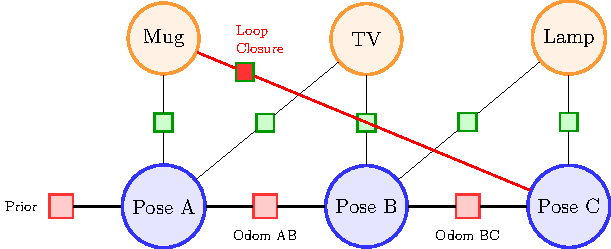
\includegraphics[width=.9\linewidth]{assets/slam_graph_3.pdf}
\caption{\label{fig:slam-graph}Bipartite graph with circles representing variable nodes and squares, the factor nodes.}
\end{figure}
\subsubsection{What is a graph?}
\label{sec:orgdb329bf}
A graph is a mathematical structure used to model
pairwise relations between objects, consisting of a set
of vertices (or nodes/dots) and a set of edges (lines)
connecting those vertices. Formally denoted as \(G =
(V,E)\), it maps how entities (vertices) are connected
(edges).

\emph{Key Concepts}
\begin{description}
\item[{Vertices \(V\)}] The nodes or dots representing objects.
\item[{Edges \(E\)}] The lines connecting two vertices,
representing relationships.
\item[{Simple Graph}] A graph with no loops (edges
connecting a vertex to itself) and no multiple edges
between the same two vertices.
\item[{Undirected Graph}] A graph where edges have no
direction, meaning the relation is two-way (e.g., \(A\)
connects to \(B\), \(B\) connects to \(A\)).
\item[{Directed Graph (Digraph)}] A graph where edges have
directions (arrows), indicating a one-way
relationship.
\item[{Adjacent Vertices}] Two vertices that are joined by
an edge.
\end{description}

\emph{Common Examples}
\begin{description}
\item[{Social Network}] People (vertices) and friendships
(edges).
\item[{GPS/ Map}] Cities (vertices) and roads (edges).
\item[{Internet}] Webpages (vertices) and hyperlinks
(directed edges).
\end{description}

Graphs are powerful for modeling non-linear, complex
networks, unlike linear data structures.
\subsubsection{What's mathematical about this?}
\label{sec:orgee9815f}

\begin{enumerate}
\item \textbf{Formality}: \(V\equiv \{ v_{i} : 0 < i \leqslant N \}\)
is a set of vertices \(v_i\) --- in its strictest
mathematical sense.  And each edge, \(e_{j}\) is a
subset of vertices, so that the set of edges
\(E\equiv \{e_j : 0 < j \leqslant M \}\) is a also a
set, albeit that of subsets of verts.
\item \textbf{Tangibility}:
\begin{description}
\item[{Degree of a node}] The number of edges connected
to a vertex.
\item[{Adjacency Matrix}] Graphs can be represented
mathematically as a matrix (a grid of numbers),
allowing for linear algebra to analyze their
properties.
\item[{Path and Cycle detection}] Mathematical formulas
exist to determine if a path exists between nodes
(Euler paths, Hamilton circuits)
\end{description}
\item \textbf{Invariants and Combinatorics}: Graph theory focuses
on invariants---properties that stay the same
regardless of how a graph is drawn.
\begin{description}
\item[{Handshaking Lemma}] A fundamental theorem stating
that the sum of all vertex degrees is always twice
the number of edges, which means the number of
odd-degree vertices must be even.
\item[{Planarity}] A graph is planar if it can be drawn
on a plane without edges crossing, a concept
deeply rooted in topology.
\end{description}
\item \textbf{Mathematical Origin}: Graph theory was invented by
Leonhard Euler to solve the Seven Bridges of
Königsberg problem.  Euler recognized that the
physical layout was irrelevant, and only the
topological structure of nodes and connections
mattered.
\item \textbf{Relationship to Reality}: While it is used to model
social networks or transport systems, the rules
governing connectivity are derived from
combinatorics, not intuition.
\end{enumerate}

In summary, graph structures are mathematical because
they are discrete systems that follow strict algebraic
and topological laws. They are used to model the real
world, but the analysis is based on mathematical
principles rather than human subjective interpretation.
\subsubsection{What's a bipartite graph?}
\label{sec:org7d0e41f}

\begin{figure}
\centering
\color{white}
\def\svgwidth{0.7\textwidth}
\input{assets/bipartite-graph.pdf_tex}
\caption{Example Bipartite Graph. Courtesy: Wikipedia}
\label{fig:bipartite-graph}
\end{figure}

A bipartite graph is a set of graph vertices
partitioned into two disjoint sets (\(V_1\) and \(V_2\))
such that every edge connects a vertex in \(V_1\) to one
in \(V_2\).  No edges exist between vertices within the
same set.  They are 2-colorable and contain no
odd-length cycles.

\emph{Key Characteristics and Properties}
\begin{description}
\item[{Vertex Partitioning}] The graph's vertices can be
divided into two independent, disjoint sets, say
\(V_{1}\) and \(V_{2}\).
\item[{Edge Restriction}] All edges must connect a vertex
from set \(V_1\) to a vertex in set \(V_2\).  No edges
are allowed between vertices within the same set.
\item[{2-Colorability}] A graph is bipartite if and only if
it can be colored using only two colors, such that no
two adjacent vertices share the same color.
\item[{Odd Cycles}] A graph is bipartite if and only if it
contains no odd-length cycles.
\item[{Complete Bipartite Graph (\(K_{m,n}\))}] A specific
type where every vertex in set \(V_1\) (size \(m\)) is
connected to every vertex in set \(V_2\) (size \(n\)).
\end{description}


\emph{Examples in Daily Life}
\begin{description}
\item[{Job Matching}] One set is employers, the other is
job openings. Edges connect employers to jobs they
offer.
\item[{Recommendation Systems}] One set of nodes is users,
the other is products. Edges represent a user
purchasing or rating a product.
\end{description}

\emph{How to Identify a Bipartite Graph?}
\begin{description}
\item[{Breadth-First Search (BFS) or Depth-First Search (DFS)}] Assign
a colour to a vertex, then its neighbours to a
different colour, alternating colours. If you find
two adjacent vertices with the same colour, it is not
bipartite.
\item[{Odd Cycle Test}] If the graph has an odd-length
cycle, it is not bipartite.
\end{description}
\subsection{Background in Optimisation Theory}
\label{sec:orge88bfde}

\subsubsection{Quadratic Programming}
\label{sec:org2da2fb1}

\begin{align*}
  f(\mathbf{x})
  &= \frac12 \mathbf{x}^{\top}Q\mathbf{x} +
    \mathbf{c}^{\top}\mathbf{x}
  && \text{\ldots Standard Quadratic Cost Function.}
  \\
  \nabla_{\mathbf{x}}f(\mathbf{x}_{*})
  &= Q\mathbf{x}_* + c = 0
  \\
  \implies \mathbf{x}_*
  &= -Q^{-1}\mathbf{c}
\end{align*}
\paragraph*{The Concept}
\label{sec:org643802e}
QP is the study of finding the minimum of a ``perfect''
quadratic bowl.  In optimization, we love quadratics
because they have a single global minimum that can be
found in exactly one step.
\paragraph*{The Mathematical Form}
\label{sec:orgb9dcfea}

A standard quadratic cost function looks like:
\(f(\mathbf{x}) = \frac{1}{2}\mathbf{x}^{\top} Q
\mathbf{x} + c^{\top} \mathbf{x}\) , where \(Q\) (The
Hessian): Defines the ``shape'' and ``stiffness'' of the
bowl; and \(\mathbf{c}\) (The Linear Trend): Defines
where the bowl is centred.
\paragraph*{The Solution}
\label{sec:org3d6d821}

To find the bottom, we take the gradient and set it to
zero: \(\nabla f(\mathbf{x}_*) = Q\mathbf{x}_* + c = 0
\implies \mathbf{x}_* = -Q^{-1}c\).
\paragraph*{Physical Intuition}
\label{sec:org619b72e}

In a Factor Graph, if all the ``springs'' were linear
(like literal metal springs following \(F=kx\)), the
entire SLAM problem would be a single QP.  We would
solve it once and be done.
\subsubsection{Gauss-Newton approximation}
\label{sec:orgeb2e891}

Let's take the context of camera re-projection error.
And the cost function be,

\begin{align*}
  f(\mathbf{x})
  &= \frac12 \mathbf{e}(\mathbf{x})^{\top}
    \mathbf{e}(\mathbf{x}) 
  && \mathbf{e}(\mathbf{x}) = \mathbf{z} -
     h(\mathbf{x})
  \\
  \nabla f(\mathbf{x})
  &= \left( \nabla \mathbf{e}(\mathbf{x}) \right)^{\top}
    \mathbf{e}(\mathbf{x}) = J^{\top}\mathbf{e}(\mathbf{x})
  && J = \nabla \mathbf{e}(\mathbf{x})
  \\
  \nabla^2 f(\mathbf{x})
  &= \underbrace{\left( \nabla \mathbf{e}(\mathbf{x})
    \right)^{\top} \nabla \mathbf{e}(\mathbf{x})}
    _{J^{\top}J} + \underbrace{ \left(\sum_i
    e_i(\mathbf{x}) \nabla^2e_i(\mathbf{x}) \right) }
    _{\text{ignored assuming } \forall i,\, e_i \to 0}
  \\
  f(\mathbf{x} + \Delta\mathbf{x})
  &\approx f(\mathbf{x}) + \nabla f(\mathbf{x})^{\top}
    \Delta \mathbf{x} + \frac12 \Delta
    \mathbf{x}^{\top} \nabla^2f(\mathbf{x}) \Delta
    \mathbf{x}
  && \text{(Taylor Expansion)}
\end{align*}
\paragraph*{The Concept}
\label{sec:orga27afaf}
The real world isn't a perfect bowl. The camera
projection \(h(x)\) is full of sines, cosines, and
divisions.  Gauss-Newton is the bridge that
\emph{approximates} a non-linear problem as a \emph{sequence of
QPs}.
\paragraph*{The Logic}
\label{sec:orgdcc816d}
Instead of trying to solve the complex landscape all at
once, we look at our current position and ask: ``If this
landscape were a quadratic bowl right here, where would
the bottom be?''

\begin{enumerate}
\item \emph{Linearise}: We take the Jacobian \(J\) (the slope) of
our error, so that \(\mathbf{c} = \nabla
   f(\mathbf{x}) = J^{\top}\mathbf{e}(\mathbf{x})\).
\item \emph{Approximate the Hessian}: Assume \(Q \approx
   J^{\top} J\).
\item \emph{Solve the QP}: Treat the neighbourhood of
\(\mathbf{x}\) as a bowl, and solve the QP,

\begin{align*}
  \mathrm{QP}(\Delta\mathbf{x})
  &= f(\mathbf{x}+\Delta\mathbf{x}) - f(\mathbf{x})
  \approx \frac12 \Delta\mathbf{x}^{\top} Q
    \Delta\mathbf{x} + \mathbf{c}^{\top}
    \Delta\mathbf{x}
  \\
  \Delta\mathbf{x}_*
  &= -Q^{-1}\mathbf{c} = -(J^{\top}J)^{-1} J^{\top}
    \mathbf{e}(\mathbf{x})
\end{align*}
\item \emph{Step}: Move to the new position, \(\mathbf{x} \gets
   \mathbf{x} + \Delta\mathbf{x}_*\) and repeat until
convergence.
\end{enumerate}
\paragraph*{Convergence Criteria}
\label{sec:orgd580548}
Practically, three things are checked to be safe.
\begin{enumerate}
\item \emph{Step delta}.  Is the change if state \(\|\Delta
   \mathbf{x}_*\|\) effectively zero.
\item \emph{Gradient delta}.  Is the slope \(\|J^{\top}
   \mathbf{e}(\mathbf{x})\|\) effectively flat?
\item \emph{Cost delta}.  Did the total error \(|f(\mathbf{x} +
   \Delta\mathbf{x}_*) - f(\mathbf{x})|\) stop decreasing?
\end{enumerate}

\begin{align*}
  \|\Delta \mathbf{x}_*\| + \|J^{\top}
  \mathbf{e}(\mathbf{x})\| + |f(\mathbf{x} +
  \Delta\mathbf{x}_*) - f(\mathbf{x})|
  &< \epsilon
\end{align*}
\subsubsection{Levenberg Marquardt Algorithm}
\label{sec:orge6c238f}

The Gauss-Newton method assumes the local ``bowl''
approximation is valid.  But what if \(J^{\top}J\) is
singular or the step \(\Delta \mathbf{x}\) is too large?
The solver overshoots, and the system diverges.  This
is where Levenberg and Marquardt stepped in.  They
added a ``damping'' term \(\lambda\) to the diagonal of the
Hessian:

\begin{align*}
  (J^{\top} J + \lambda \mathbf{I}) \Delta \mathbf{x}_*
  &= -J^{\top} \mathbf{e}(\mathbf{x}) \\ \text{or,
  }\quad \Delta \mathbf{x}_*
  &= -(J^{\top} J + \lambda I) ^{-1} J^{\top}
    \mathbf{e}(\mathbf{x})
\end{align*}

The beauty of LM is that it dynamically slides between
two optimization strategies based on the value of
\(\lambda\):
\paragraph*{When \(\lambda\) is large (The Gradient Descent Limit)}
\label{sec:org5558c43}

\(\Delta \mathbf{x}_* \approx
-\mathbf{J}^{\top} \mathbf{e} / \lambda\). \\
This is a small step in the direction of the steepest
descent. It is stable but slow. We use this when our
quadratic approximation is poor (the error is
increasing).
\paragraph*{When \(\lambda\) is small (The Quadratic Program Limit)}
\label{sec:org0f4ed08}

\(\Delta \mathbf{x}_* \approx (J^{\top}J)^{-1}J^{\top}
\mathbf{e}(\mathbf{x})\). \\
This is the Gauss-Newton step. It is unstable far from
the minimum but lightning-fast (quadratic convergence)
near the minimum.
\paragraph*{Comparison with Gauss-Newton}
\label{sec:org83e072c}
\begin{center}
\begin{tabularx}{\textwidth}{lXX}
\hline
\textbf{Feature} & \textbf{Standard QP} & \textbf{LM Algorithm}\\
\hline
Curvature & Exact Hessian (\(H\)) & Approximate Hessian, \emph{i.e.} (\(J^{\top}J+\lambda I\))\\
Trust Region & Infinite (assumes the bowl is real) & Finite (constrained by \(\lambda\))\\
Step Calculation & One-shot Matrix Inversion & Iterative, ``Solve, check error, and adjust \(\lambda\)''\\
Global Goal & Find the bottom of the bowl & Move between local bowls until tension is zero\\
\end{tabularx}
\end{center}
\paragraph*{Strategy for tuning \(\lambda\)}
\label{sec:org077ff8d}
In SLAM, we use LM because we are constantly moving
from ``I have no idea where I am'' to ``I am almost
certain where I am.''

\begin{enumerate}
\item \emph{Start}: \(\lambda\) is high. We take cautious,
gradient-like steps to move toward the general area
of the minimum.
\item \emph{Middle}: As the error decreases, we decrease
\(\lambda\). The ``springs'' of our Factor Graph start
behaving more like the Quadratic Model we built.
\item \emph{End}: \(\lambda\) becomes near-zero. We take a final,
massive ``Gauss-Newton leap'' to the exact center of
the minimum, providing the millimeter-precision
needed for AR.
\end{enumerate}
\section{CV}
\label{sec:org267bc1b}
To put this in perspective, if \textbf{SLAM} is the ``Inner
Ear'' and ``Memory'' of an AR system (handling balance,
movement, and mapping), then \textbf{Computer Vision (CV)} is
the ``Eyes'' and ``Intelligence.''

While SLAM tells you \emph{where} you are, CV tells you
\emph{what} you are looking at.  Together, they bridge the
gap between a raw video feed and a persistent digital
world.
\subsection{The CV-SLAM Symbiosis}
\label{sec:org39c0523}
It is common to say AR = CV + SLAM. Here is how they divide the labor:

\begin{description}
\item[{SLAM}] Focuses on \textbf{geometry}. It calculates the
transformation matrix between the camera and the
world.  It doesn't care if a feature is a ``chair'' or
a ``rock''---it only cares that the feature is a 3D point
at \((x, y, z)\).
\item[{Computer Vision}] Focuses on \textbf{semantics and
perception}.  It interprets the image to provide
context, constraints, and interaction points for the
AR content.
\end{description}
\subsection{Key CV Tasks in AR}
\label{sec:orgb796748}
Beyond just finding points for SLAM, CV performs
several critical functions that make AR feel ``real'':
\subsubsection{Image Recognition \& Tracking}
\label{sec:orgceb66ee}
This is the ability to detect a specific 2D image (like
a movie poster or a QR code) and use it as a ``Trigger.''
\begin{description}
\item[{How it works}] CV extractors (like SIFT or ORB)
create a ``fingerprint'' of the image and match it
against a database.
\item[{AR Result}] When you point your phone at a specific
book cover, a 3D animation pops out of it.
\end{description}
\subsubsection{Object Detection \& Labeling}
\label{sec:org01a0b94}
CV identifies real-world objects (cars, people,
furniture) using Deep Learning (CNNs).

\emph{Plausible AR Result}: A ``Terminator-style'' HUD that
labels the people in your field of view or recognizes a
specific model of a machine to overlay repair
instructions.
\subsubsection{Semantic Segmentation}
\label{sec:org9d490bf}
This is the process of labeling every single pixel in a
frame (e.g., ``this pixel is grass,'' ``this pixel is
sky'').

\emph{Plausible AR Result}: This allows for \textbf{Occlusion}.  If
the CV knows the pixels in the centre of the screen are
a ``Human,'' the AR system can hide a digital monster
\emph{behind} that person instead of just rendering it on
top of them.
\subsection{Scene Understanding: The ``Physics'' of CV}
\label{sec:org61b4548}
For an AR object to look like it belongs in the room,
CV must extract environmental data that SLAM usually
ignores:

\begin{description}
\item[{Plane Detection}] CV identifies flat surfaces
(floors, tables, walls). This is where the \textbf{Quadratic
Program} of our SLAM system meets the ``Logic'' of CV.
The system identifies a cluster of 3D points that are
co-planar and ``snaps'' a virtual floor to them.
\item[{Light Estimation}] CV analyzes the highlights and
shadows in the camera feed to determine the direction
and intensity of real-world light.
\end{description}

\emph{Plausible AR Result}: A virtual dinosaur casts a
shadow that matches the shadows of the real furniture.
\subsection{The ``Frontend'' of the Pipeline (Feature Extraction)}
\label{sec:org8815d52}
Computer Vision provides the raw materials for
SLAM.  Before you can run a Gauss-Newton optimization,
CV must:
\begin{enumerate}
\item \emph{Detect}: Find ``interesting'' pixels (corners,
blobs).
\item \emph{Describe}: Turn those pixels into a math vector
(Descriptor).
\item \emph{Match}: Compare descriptors between Frame A and
Frame B.
\end{enumerate}

If the CV ``Front-end'' fails to find good matches (due
to motion blur or low light), the SLAM ``Back-end'' (the
optimizer) has no data to work with, and the AR
``drifts.''
\section{Summary: The Two Pillars}
\label{sec:orgf6d8b20}
\begin{center}
\begin{tabularx}{\linewidth}{llX}
\textbf{Tech} & \textbf{Primary Goal} & \textbf{Math/Tooling}\\
\hline
SLAM & Spatial Consistency & Factor Graphs, Gauss-Newton, IMU Integration\\
CV & Context \& Realism & Neural Networks, Feature Matching, Photometry\\
\end{tabularx}
\end{center}

In modern AR, the line is blurring. We now have
\textbf{Semantic SLAM}, where the ``Factor Graph'' doesn't
just contain points, but recognized objects (e.g., ``The
factor between Pose A and Pose B must respect the fact
that Pose A is looking at a `Table'''). 

Does this distinction help you see CV as the
``Intelligence'' layer that sits on top of the
``Geometric'' foundation of SLAM?
\end{document}
